\documentclass{beamer}
\usetheme{metropolis} 
\usepackage{listings}
\usepackage{xcolor}
\definecolor{myBlue}{RGB}{0, 0, 180}
\definecolor{myGreen}{RGB}{34, 139, 34}
\definecolor{myRed}{RGB}{180, 0, 0}
\definecolor{myGray}{RGB}{96, 96, 96}
\lstset{ 
    language=Python,
    basicstyle=\ttfamily\tiny,
    keywordstyle=\color{myBlue},
    commentstyle=\color{myGreen},
    stringstyle=\color{myRed},
    showstringspaces=false,
    numberstyle=\tiny\color{myGray},
    stepnumber=1,
    numbersep=5pt,
    frame=single,
    breaklines=true,
    breakatwhitespace=true,
    tabsize=4,
    captionpos=b
}
\title{Chapter 2: Multi-armed Bandits}
\date{\today}
\author{Gabe Sekeres}
\institute{Cornell University}
\begin{document}

  \maketitle
  
\begin{frame}{Introduction}
	\begin{itemize}
		\item We have a simple environment: 10 arms, where each arm $k_i$ is defined by \[k_i \sim \mathcal{N}(q_i,1) \quad \text{ where } q_i \sim \mathcal{N}(0,1), i = 1,\dots,10\]
		\item The text considers three different bandit algorithms: $\varepsilon$-greedy, upper confidence bound (UCB), and gradient
		\item Here, I show only the code for $\varepsilon$-greedy. I did replicate the others in Julia, the full code is 
	\end{itemize}
\end{frame}
  
 \begin{frame}{Reward Distributions (fig. 2.1)}
 	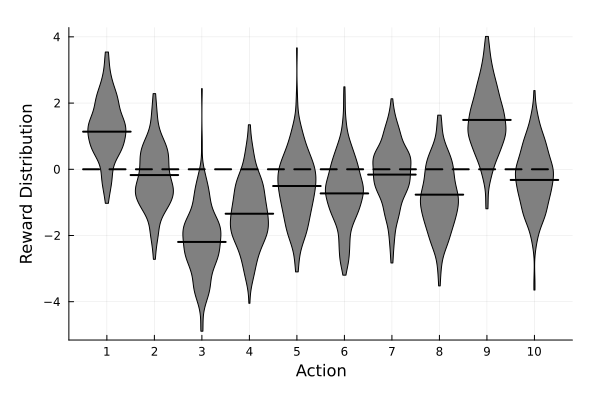
\includegraphics[width=11cm]{ten_armed_testbed_violin.png}
 \end{frame}
  
  \begin{frame}{Epsilon Reward Comparison (fig. 2.2a)}
  	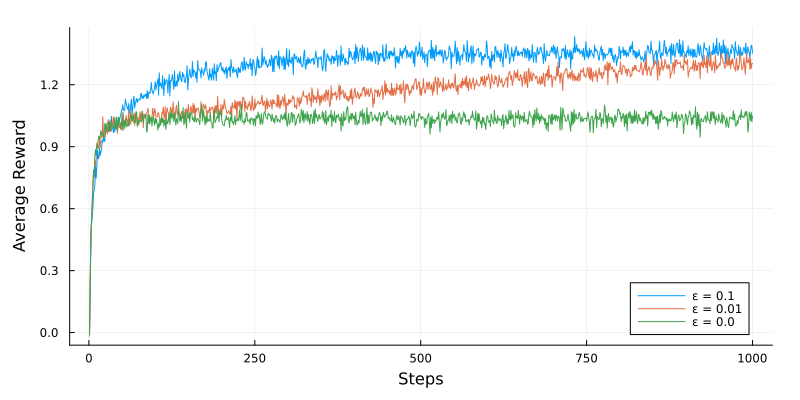
\includegraphics[width=11cm]{ten_armed_testbed_epsilon_greedy.png}
  \end{frame}
  
    \begin{frame}{Epsilon Action Comparison (fig. 2.2b)}
  	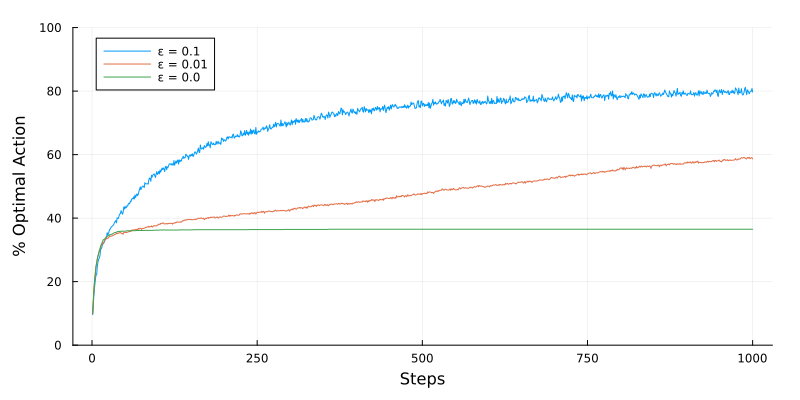
\includegraphics[width=11cm]{ten_armed_testbed_epsilon_optimal.png}
  \end{frame}
  
\begin{frame}{Optimistic vs. Realistic (fig. 2.3)}
	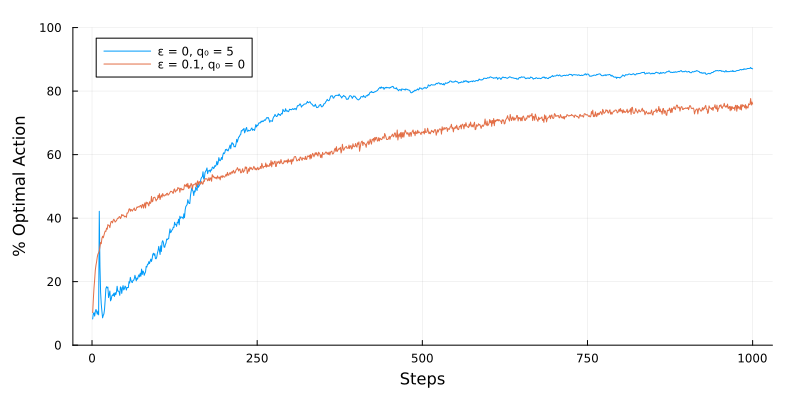
\includegraphics[width=11cm]{ten_armed_testbed_optimistic.png}
\end{frame}
\begin{frame}{UCB vs. Epsilon (fig. 2.4)}
	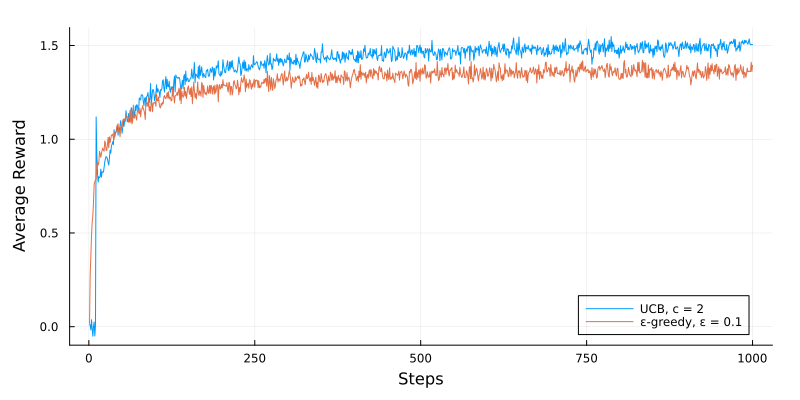
\includegraphics[width=11cm]{ten_armed_testbed_ucb.png}
\end{frame}
\begin{frame}{Gradient Baseline Comparison (fig. 2.5)}
	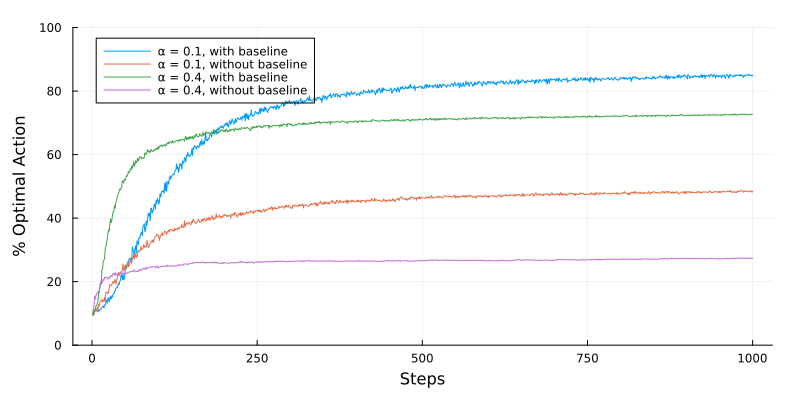
\includegraphics[width=11cm]{ten_armed_testbed_gradient.png}
\end{frame}
\begin{frame}{Full Bandit Comparison (fig. 2.6)}
	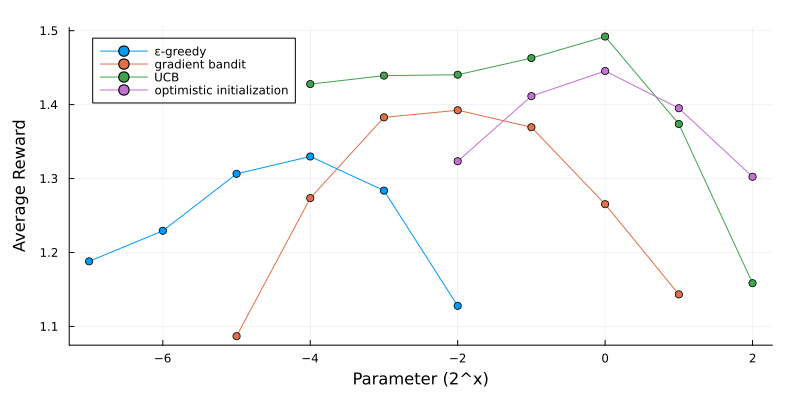
\includegraphics[width=11cm]{ten_armed_testbed_comparison.png}
\end{frame}
  
  
  
\end{document}